% The document class supplies options to control rendering of some standard
% features in the result.  The goal is for uniform style, so some attention 
% to detail is *vital* with all fields.  Each field (i.e., text inside the
% curly braces below, so the MEng text inside {MEng} for instance) should 
% take into account the following:
%
% - author name       should be formatted as "FirstName LastName"
%   (not "Initial LastName" for example),
% - supervisor name   should be formatted as "Title FirstName LastName"
%   (where Title is "Dr." or "Prof." for example),
% - degree programme  should be "BSc", "MEng", "MSci", "MSc" or "PhD",
% - dissertation title should be correctly capitalised (plus you can have
%   an optional sub-title if appropriate, or leave this field blank),
% - dissertation type should be formatted as one of the following:
%   * for the MEng degree programme either "enterprise" or "research" to
%     reflect the stream,
%   * for the MSc  degree programme "$X/Y/Z$" for a project deemed to be
%     X%, Y% and Z% of type I, II and III.
% - year              should be formatted as a 4-digit year of submission
%   (so 2014 rather than the accademic year, say 2013/14 say).


\documentclass[ % the name of the author
                    author={Callum Pearce},
                % the name of the supervisor
                supervisor={Dr. Neill Campbell},
                % the degree programme
                    degree={MEng},
                % the dissertation    title (which cannot be blank)
                     title={How effective are Temporal difference learning methods for reducing the number of zero contribution light paths while still accurately approximating Global Illumination in Path tracing?},
                % the dissertation subtitle (which can be blank)
                  subtitle={},
                % the dissertation     type
                      type={research},
                % the year of submission
                      year={2019} ]{dissertation}

\begin{document}

% =============================================================================

% This section simply introduces the structural guidelines.  It can clearly
% be deleted (or commented out) if you use the file as a template for your
% own dissertation: everything following it is in the correct order to use 
% as is.

\section*{Prelude}
\thispagestyle{empty}

A typical dissertation will be structured according to (somewhat) standard 
sections, described in what follows.  However, it is hard and perhaps even 
counter-productive to generalise: the goal is {\em not} to be prescriptive, 
but simply to act as a guideline.  In particular, each page count given is
important but {\em not} absolute: their aim is simply to highlight that a 
clear, concise description is better than a rambling alternative that makes
it hard to separate important content and facts from trivia.

You can use this document as a \LaTeX-based~\cite{latexbook1,latexbook2} 
template for your own dissertation by simply deleting extraneous sections
and content; keep in mind that the associated {\tt Makefile} could be of
use, in particular because it automatically executes  to 
deal with the associated bibliography.  

You can, on the other hand, opt {\em not} to use this template; this is a 
perfectly acceptable approach.  Note that a standard cover and declaration 
of authorship may still be produced online via
\[
\mbox{\url{http://www.cs.bris.ac.uk/Teaching/Resources/cover.html}}
\]

% =============================================================================

% This macro creates the standard UoB title page by using information drawn
% from the document class (meaning it is vital you select the correct degree 
% title and so on).

\maketitle

% After the title page (which is a special case in that it is not numbered)
% comes the front matter or preliminaries; this macro signals the start of
% such content, meaning the pages are numbered with Roman numerals.

\frontmatter

% This macro creates the standard UoB declaration; on the printed hard-copy,
% this must be physically signed by the author in the space indicated.

\makedecl

% LaTeX automatically generates a table of contents, plus associated lists 
% of figures, tables and algorithms.  The former is a compulsory part of the
% dissertation, but if you do not require the latter they can be suppressed
% by simply commenting out the associated macro.

\tableofcontents
\listoffigures
\listoftables
\listofalgorithms
\lstlistoflistings

% The following sections are part of the front matter, but are not generated
% automatically by LaTeX; the use of \chapter* means they are not numbered.

% -----------------------------------------------------------------------------

\chapter*{Executive Summary}

\begin{comment}
{\bf A compulsory section, of at most $1$ page} 
\vspace{1cm} 

\noindent
This section should pr\'{e}cis the project context, aims and objectives,
and main contributions (e.g., deliverables) and achievements; the same 
section may be called an abstract elsewhere.  The goal is to ensure the 
reader is clear about what the topic is, what you have done within this 
topic, {\em and} what your view of the outcome is.

The former aspects should be guided by your specification: essentially 
this section is a (very) short version of what is typically the first 
chapter.  Note that for research-type projects, this {\bf must} include 
a clear research hypothesis.  This will obviously differ significantly
for each project, but an example might be as follows:

\begin{quote}
My research hypothesis is that a suitable genetic algorithm will yield
more accurate results (when applied to the standard ACME data set) than 
the algorithm proposed by Jones and Smith, while also executing in less
time.
\end{quote}

\noindent
The latter aspects should (ideally) be presented as a concise, factual 
bullet point list.  Again the points will differ for each project, but 
an might be as follows:

\begin{quote}
\noindent
\begin{itemize}
\item I spent $120$ hours collecting material on and learning about the 
      Java garbage-collection sub-system. 
\item I wrote a total of $5000$ lines of source code, comprising a Linux 
      device driver for a robot (in C) and a GUI (in Java) that is 
      used to control it.
\item I designed a new algorithm for computing the non-linear mapping 
      from A-space to B-space using a genetic algorithm, see page $17$.
\item I implemented a version of the algorithm proposed by Jones and 
      Smith in [6], see page $12$, corrected a mistake in it, and 
      compared the results with several alternatives.
\end{itemize}
\end{quote}
\end{comment}

In the field of Computer Graphics, Path tracing is an algorithm which 
accurately approximates global illumination in order to produce 
photo-realistic images. Path tracing has traditionally been known to 
trade speed for image quality. This is due to the lengthy process of accurately 
finding each pixels colour, whereby many light rays are 
fired through each pixel into scene, then directions for each ray are 
continually sampled until it intersects with a light source. Due to 
this, a variety of Importance sampling algorithms have been designed 
to avoid sampling directions which lead to rays contributing no light 
to the rendered image. The paths formed by sampling rays in these 
directions are known as zero contribution light paths. By not sampling 
zero contribution light paths, it is possible to significantly reduce 
the noise in rendered images using the same number of sampled rays per 
pixel in path tracing\\

Recently a Temporal Difference learning method was used by Nvidia to
achieve impressive results in Importance sampling within a Path tracer.
The algorithm essentially learns which directions light is coming from for
a given point in the scene. It then uses importance sampling to favour shooting
rays stored in those directions, reducing the number of zero contribution light paths
sampled. With this success, there is plenty of potential to experiment with
other Temporal Difference learning methods, particularly Deep Q-Learning.
It is also important to assess both of these methods on their ability to 
accurately approximate Global Illumination to produce photo-realistic images.
From this, my goal is to investigate the ability of two different temporal
difference learning algorithms ability to reduce the number of zero contribution
light paths in path tracing, whilst still accurately approximating global illumination.
More specifically, the first temporal difference learning method will be that proposed
by Nvidia, and the second will be my designed Neural-Q path tracing algorithm.
I will be comparing these two methods in order to test the following hypothesis:

\begin{quote}
The Neural-Q  path tracer is further able to reduce
the number of zero contribution light paths than an Expected SARSA
Path tracer proposed by Nvidia, whilst still accurately simulating Global Illumination.
\end{quote}

\noindent
\textbf{Outcomes}
\begin{itemize}
\item Which is better able to reduce the number of zero contribution light paths expected SARSA or Deep Q-learning
\item Can Expected SARSA learning handle multiple lights well in a scene \& deep q-learning
\end{itemize}

\noindent
\textbf{Main areas of work}
\begin{itemize}
\item I have written $x$ lines of code to build a  Path tracing engine from scratch which supports a variety of GPU accelerated Path tracing algorithms I have experimented with.

\item I have spent $x$ hours researching into the field of efficient light transport simulation for ray-tracing techniques.

\item I have spent $x$ hours researching into Reinforcement learning, particularly Temporal Difference learning and Deep Reinforcement learning, neither of which I have been taught before.

\item I spent $x$ hours implementing and validating the on-line Expected SARSA Path tracing algorithm proposed by Nvidia, which required me to implement the Irradiance Volume data structure as a prerequisite.

\item I have spent $x$ hours designing, implementing and analysing my own on-line Deep Q-learning Path tracing algorithm, along with a neural network architecture
designed for the algorithm.

\end{itemize}


% -----------------------------------------------------------------------------

\chapter*{Supporting Technologies}

\begin{comment}
{\bf A compulsory section, of at most $1$ page}
\vspace{1cm} 

\noindent
This section should present a detailed summary, in bullet point form, 
of any third-party resources (e.g., hardware and software components) 
used during the project.  Use of such resources is always perfectly 
acceptable: the goal of this section is simply to be clear about how
and where they are used, so that a clear assessment of your work can
result.  The content can focus on the project topic itself (rather,
for example, than including ``I used \mbox{\LaTeX} to prepare my 
dissertation''); an example is as follows:

\begin{quote}
\noindent
\begin{itemize}
\item I used the Java {\tt BigInteger} class to support my implementation 
      of RSA.
\item I used a parts of the OpenCV computer vision library to capture 
      images from a camera, and for various standard operations (e.g., 
      threshold, edge detection).
\item I used an FPGA device supplied by the Department, and altered it 
      to support an open-source UART core obtained from 
      \url{http://opencores.org/}.
\item The web-interface component of my system was implemented by 
      extending the open-source WordPress software available from
      \url{http://wordpress.org/}.
\end{itemize}
\end{quote}
\end{comment}


\begin{enumerate}
\item I used the \verb|SDL2|  library for displaying and saving rendered 
images from my Path tracing engine.

\item I used the \verb|OpenGL| mathematics library to support low level 
operations in my Path tracing engine. It includes GPU accelerated 
 implementations for all of its functions.
 
\item I used the \verb|CUDA Toolkit 10.1| parallel computing platform for
 accelerating Path tracing algorithms. This means the \verb|CUDA nvcc|
 compiler must be used to compile my Path tracing engine.

\item All experiments were run on my own desktop machine with an
Nvidia \verb|1070Ti| GPU, Intel \verb|i5-8600K| CPU and $16$GB of RAM.

\item I used the C++ API for the \verb|Dynet| neural network framework 
to implement all of my Neural Network code as it is able to be compiled
by the \verb|CUDA| compiler.
\end{enumerate}

% -----------------------------------------------------------------------------

\chapter*{Notation and Acronyms}

\begin{comment}
{\bf An optional section, of roughly $1$ or $2$ pages}
\vspace{1cm} 

\noindent
Any well written document will introduce notation and acronyms before
their use, {\em even if} they are standard in some way: this ensures 
any reader can understand the resulting self-contained content.  

Said introduction can exist within the dissertation itself, wherever 
that is appropriate.  For an acronym, this is typically achieved at 
the first point of use via ``Advanced Encryption Standard (AES)'' or 
similar, noting the capitalisation of relevant letters.  However, it 
can be useful to include an additional, dedicated list at the start 
of the dissertation; the advantage of doing so is that you cannot 
mistakenly use an acronym before defining it.  A limited example is 
as follows:
\end{comment}

\begin{quote}
\noindent
\begin{tabular}{lcl}
TD learning    &:    & Temporal Difference learning\\
\end{tabular}
\end{quote}

% -----------------------------------------------------------------------------

\chapter*{Acknowledgements}

{\bf An optional section, of at most $1$ page}
\vspace{1cm} 

\noindent
It is common practice (although totally optional) to acknowledge any
third-party advice, contribution or influence you have found useful
during your work.  Examples include support from friends or family, 
the input of your Supervisor and/or Advisor, external organisations 
or persons who  have supplied resources of some kind (e.g., funding, 
advice or time), and so on.

\subsection{Plan}
\begin{enumerate}
\item Carl Henrik Ek - Validating my understanding of deep reinforcement learning
\item Neill Campbell - Deep reinforcement learning strategy
\end{enumerate}

% =============================================================================

% After the front matter comes a number of chapters; under each chapter,
% sections, subsections and even subsubsections are permissible.  The
% pages in this part are numbered with Arabic numerals.  Note that:
%
% - A reference point can be marked using \label{XXX}, and then later
%   referred to via \ref{XXX}; for example Chapter\ref{chap:context}.
% - The chapters are presented here in one file; this can become hard
%   to manage.  An alternative is to save the content in seprate files
%   the use \input{XXX} to import it, which acts like the #include
%   directive in C.

\mainmatter

% -----------------------------------------------------------------------------

\chapter{Contextual Background}
\label{chap:context}

% I don't like this, needs to be more like the opening of a book chapter 

This chapter explains on a high level what path tracing is and how it accurately 
simulates light transport. Then importance sampling ray directions in light
transport simulation is discussed, and how it can potentially reduce the number 
of zero contribution light paths and the associated benefits with this. Temporal 
difference learning as a branch of reinforcement learning is then introduced, 
along with how it can be used in importance sampling ray directions towards 
light sources. With a conceptual overview of theory my work is based on, I take 
a look at recent work which contributes to real-time accurate light transport 
simulation which my work aims to contribute to. Finally, an overview of the 
objectives and significant challenges of my investigation are described.


\section{Path Tracing for Light Transport Simulation}
Path Tracing is a Monte Carlo method for rendering photo-realistic images of 3D 
scenes by accurately approximating global illumination \cite{christensen2016path}.
Figure \ref{} summarises on a high level how forward Path tracing produces a 
2D image of a 3D scene. For each pixel multiple rays are shot from the camera through the 
pixel and into the scene. Any ray which intersects with an area light terminates, 
otherwise a new direction is sampled for the ray and it is fired again. This process 
is repeated until all rays have intersected with an area light, at which point the pixel 
colour value can  be found by averaging the colour estimate of each ray fired 
through that pixel. Each rays colour estimate is calculated based on the material 
surface properties it intersects with before intersecting with the light and the
intersected area lights properties. The more rays shot through each pixel (also 
known as samples per pixel), the more visually accurate the rendered image 
becomes, but at a higher computational cost.\\

% Figure of path tracing, needs to clearly label what a light transport path is

Path tracing simulates global illumination, meaning it accounts for both direct and 
indirect illumination. Direct illumination being rays of light emitted from a light 
source, which reflect off exactly one surface before reaching the camera in the 
scene. Whereas indirect illumination are ray of light which reflect 2 or times before
reaching the camera. In \ref{}, an identical scene is shown with only direct illumination
(left) and the other with global illumination (right). The globally illuminated scene displays
a range of effects due to Path tracings ability to accurately simulate light transport, 
which is not the case for the directly illuminated scene. Where light transport simulation
refers to firing and summing up the contributions of light transport paths that connect from the
camera to light sources \cite{keller2016path}, such as those displayed in \ref{}. For 
example, effects such as (a) colour bleeding, (b) soft shadows, and (c) indirect diffuse lighting
are a product of accurate light transport simulation. \\

% Put and image of the scene with a big light on the write, 4096 spp and 1 bounce on the left and 4096 spp 1000 bounces on the right

Light transport simulation methods are able to produce 
many complex light transport effects by a simple single pass of a rendering algorithm.
This allows artists to increase productivity and perform less manual image tweaking
in the production of photo-realistic images. Due to this, the Computer Graphics 
industry has seen a large resurgence in research and usage of light transport simulation 
rendering methods in the past decade \cite{krivanek2014recent}. \\

My work in this thesis focuses on developing and assessing importance sampling 
techniques using Temporal Difference learning methods for light transport simulation 
in forward Path tracing. In particular, More specifically,
for any intersection point in a 3D scene, I attempt to create an AI agent that learns 
and samples in  directions light is coming from, reducing the total number of 
zero contribution light paths. A zero contribution light path is one whose 
estimated colour values are almost zero for all $(R,G,B)$ components, hence,
they contribute almost no visible difference to the rendered image. We should 
instead focus our sampling on light paths which do contribute to the image,
reducing the noise in pixel values and bringing them closer to their true 
values for the same number of sampled rays per pixel. Meaning, Importance 
sampling can reduce the number of rays needed to be sampled per pixel in 
order to receive a photo-realistic (also known as converged) image from Path 
tracing. An example of this reduction in noise can be see in \ref{}, where the 
naive forward Path tracing algorithms output is compared to Nvidia's on-line
reinforcement learning Path tracer using Importance sampling. Note, any 
light transport simulation algorithm can benefit from the Temporal DIfference learning
schemes which will be described \cite{jensen1996global, keller2016path}, 
as they are all derived from what is known as the rendering equation. This equation
is used as a mathematical basis of modelling light transport.\\

% Comparison between importance sampling and path tracing with the same number of samples

It is paramount that Importance sampling Path tracing algorithms continue to accurately
simulates global illumination in order to produce photo-realistic images in a single
rendering pass, as this is the major selling point of Path tracing over other 
methods. Therefore, I will also be assessing the accuracy of the global
illumination approximation made by the Importance sampling algorithms compared
to that of the naive forward Path tracing algorithm.

\section{Temporal Difference Learning for Importance Sampling Ray Directions}

There are three important unanswered questions up to this point; a) what is temporal
difference learning?  b) How can temporal difference learning methods be 
used to importance sample new ray directions for a given intersection point in 
the scene? c) Why use temporal difference learning methods over other Importance 
sampling methods to do so? 

\subsection{What is Temporal Difference learning?}
Temporal difference learning, which I will refer to from 
here on as TD learning, are a set of model free Reinforcement learning methods. 
Firstly, Reinforcement learning is the process of an AI agent learning what is the 
best action to take in any given state of the system it exists within, in order to 
maximise a numerical reward signal \cite{sutton2011reinforcement}.
The AI agent is not told which actions are  best to take in a given state, but
 instead it must learn which ones are by trialling them and observing the reward 
signal. Actions taken may not only affect the immediate 
reward, but all subsequent rewards received for taking future actions. For 
example, picture a robot rover whose duty it is to explore the surrounding area 
as much possible. A state in this case is a position in the world it is exploring, 
and its action are the directions to move in for a given distance. If it discovers 
a new area, it receives a positive reward signal. Now, if the robot chooses to 
explore a given area it may not be able to get back from, say a canyon, the 
robot is limited to searching areas reachable from the canyon. Hence, all 
subsequent reward signals are limited to what can be received from exploration 
of the canyon, compared to not entering the canyon and exploring areas which 
can be returned from first.

As mentioned TD learning methods are model free methods, meaning the methods 
do not require a model of the system dynamics they are placed in, instead they
 learn over time by interacting with the system. In other words, they learn from 
 raw experience  \cite{sutton2011reinforcement}. TD methods update their current
estimates based on a combination of data received from interacting with the 
environment, and partly on their current learned estimates without waiting for the 
final outcome of events, this is known as bootstrapping. To illustrate the concept 
of bootstrapping, imagine you are driving home from work and you wish to estimate 
how long it will take you get home. By following a TD learning method, if you hit 
traffic you can update your current estimate of the time it takes you to drive home
based on this new data, and your pre-existing estimate. Whereas compared to 
another set of Reinforcement learning methods known as Monte Carlo methods, 
you would have to wait until you got home to update your current estimate of how 
long it takes to get home from work. Meaning you have to wait for the final outcome
before learning can begin, which is not the case for TD learning.

\subsection{Temporal Difference learning methods for Efficient Light Transport Simulation}

One of my main aims to reduce the number of zero contribution light paths sampled 
in Path tracing by the use of TD learning methods. In order to do so I must formulate 
the problem a reinforcement learning problem, which is done in detail in Chapter
\ref{chap:technical}. However for a conceptual overview it suffices to explain what a 
state, action, and reward signal will be in the case of light transport simulation within 
Path tracing:

\begin{itemize}

\item \textbf{State}: A 3D intersection position in the scene for a given ray to sample 
the rays next direction from. 

\item \textbf{Action}: Firing the ray in a given direction (3D vector) from the current 
state.

\item \textbf{Reward Signal}: The amount of light incident from the direction the ray 
was sampled in.

\end{itemize}

In this reinforcement learning setting, we can use TD-learning methods to create 
an AI agent which learns by taking different actions in different states and observes 
their reward signals to find out for each state which actions have the highest valuations.
By then converting the action space into a probability distribution weighted by each
actions learned valuation, the AI agent will more likely sample non-zero contribution 
light paths, reducing noise in rendered images. Note, the term valuation means the 
total expected reward for taking a given action, meaning valuation not only accounts 
for the immediate reward, but the expected reward for taking all future actions to come 
until the ray intersects with a light. Also, for the proposed AI agent, current actions 
can affect future rewards, as when the ray intersects a surface it looses some energy. 
Therefore, future rewards received after many intersections will be discounted 
compared to the reward of received immediately to match this behaviour. This means 
the agent will aim to minimise the average number of intersection a ray makes before 
intersecting with a light source, making it a good metric to test evaluate against to 
determine how well the AI agent is performing.

\subsection{Why use Temporal Difference Learning for Importance Sampling?}

Traditional Importance sampling techniques for Path tracing do not take into account 
the visibility of the object from light. A light blocker is shown in \ref{}, where the 
blocking object stops rays from directly reaching the light. Due to the unknown 
presence of blockers, traditional importance sampling methods can fail to avoid 
sampling zero contribution light paths. Therefore, scenes which are significantly 
affected by blockers will not receive the benefits from traditional Importance sampling 
and can even benefit more from an uniform sampling scheme 
\cite{ramamoorthi2012theory}.\\

% vector art to display the concept of a light blocker

Temporal difference learning methods are able to solve this problem 
\cite{dahm2017learning}. As the AI agent described in the previous section learns 
which directions light is coming from in the scene and concentrates its sampling 
towards these directions. Directions leading to blockers will have a low value, 
hence it is unlikely the AI agent will sample rays in these directions.\\

\section{Motivation}

Rendering time of my graphics engine is not something I have tried to heavily 
optimise. I instead focus on producing higher quality images using the same 
number of samples per pixel in light transport simulation in hope that future 
work will find ways of optimising my methods for speed. Therefore, my work 
still aims to contribute to the wider goal seen in computer graphics to use 
accurate light transport simulation in the rendering of photo-realistic images 
for complex scenes in real-time.  Speeding up the methods I use is a large 
topic in itself, requiring a deep investigation into the best software, hardware, 
and parallel programming paradigms to use.\\

\subsection{Real time Rendering using Accurate Light Transport Simulation}
The motivation for using accurate light transport simulation in real-time 
comes from the clear superior visual quality of images rendered using this 
techniques, compared to that of scanline methods which are currently used. 
Where scanline rendering, also known as rasterizing, is the current computer 
graphics industry standard method for real-time rendering. Not only are 
renders for a wide range of scenes clearly superior from methods which 
accurately simulate light transport, but they also scale far better with the 
number of polygons used to build the scenes surfaces. Therefore, scanline 
rendering for scenes with extremely complex geometry in real-time is currently 
not and option. Accurate light transport simulation methods therefore have 
great potential to be used in ultra realistic simulations for applications such 
as scenario planning and virtual reality learning environments \cite{pan2006virtual}. 
Also, many games sell realism as one of their most important features, therefore 
developing photo-realistic graphics in real-time has clear economic incentive for 
the video games industry which was valued at over \$$136$ by the end of 2018 
\cite{bloomberg.com}. An economic incentive can also be seen for the film
industry, where reductions in render times lead to a direct saving on compute 
time, as well as the hardware required to render full length films.

\subsection{Recent Developments}
Due to the incentives, a large amount of research and investment has been focused 
on purpose built hardware and Deep learning  post-processing methods in an 
attempt to bring accurate light transport simulation into real-time. NVIDIA's 
Turing Ray Tracing Technology \cite{nvidia_turing_architecture_whitepaper_2018} 
represents a significant leap in the hardware to support light transport simulation. 
It allows for real-time graphics engines to be a hybrid of both scanline rendering, 
and ray-tracing. The 20 series Turing GPU architecture has significantly improved 
the speed of ray-casting for light transport simulation, and has the capacity for  
simulating 10 Giga Rays per second. However, using this hardware alone with 
current rendering methods is not enough to perform accurate light transport 
simulation for complex scenes in real-time.\\

Post-processing methods are designed to take a noisy input image produced by a 
render which simulates light transport, and then reconstruct the image to remove 
the noise present in the image. Generally these methods rely on pre-trained deep 
neural networks to reconstruct the image far quicker then it would take for the 
renderer to produce an image of the same visual quality \cite{bako2017kernel}. 
Once again NVIDIA has made significant advancements in this area with NVIDIA 
OptiX AI Accelerated Denoiser, which is based on their newly designed recurrent 
denoising autoencoder \cite{chaitanya2017interactive}. OptiX has been successfully 
integrated in to many of the top rendering engines which accurately simulate light
transport, such as RenderMan \cite{christensen2018renderman} and Arnold 
\cite{georgiev2018arnold}. Whilst post-processing has significantly reduced the 
number of samples required to render photo-realistic images, there is still more 
work to be done to produce these images in real-time.\\

By using importance sampling by TD learning to reduce the number of samples 
required for accurate light transport simulation, the same standard of noisy 
image can be fed into an AI accelerated denoiser with fewer samples per pixel 
in light transport simulation. Running a rendering engine optimised in this way on 
purpose built hardware could make accurate light transport simulation for 
rendering photo-realistic images closer than it ever has been to real-time.

\section{Challenges and Objectives}

% Needs work

As previously mentioned, there already exists an example of TD learning used 
for importance sampling ray directions in a forward Path tracer \cite{dahm2017learning}. 
However, further methods of analysis need to be conducted upon this new 
method to determine its performance for reducing the number of zero contribution l
ight paths for different scenes with different settings. It is difficult to assess this as 
there are infinitely many scenes the method can be used to render, so coming to a 
clear conclusion is difficult. Another difficult task is that of designing an algorithm 
for an AI agent to learn what are the favourable directions to sample in a scene are 
using the deep Q-learning method. This includes some important unanswered 
questions, such as; is it possible for a deep neural network to model all Q values for 
a continuous scene space? If so, what is a suitable network architecture? All of 
which I will describe in more depth in Chapter \ref{chap:deep-q}. Then the actual 
task of implementing such an algorithm in a graphics engine written from scratch 
is non-trivial due to the technologies which will need to be combined together. 
The algorithm must also run fast enough to collect large amounts of data from, 
otherwise a justified conclusion on its performance cannot be made. Therefore, 
the algorithm will have to be parallelized and run on a GPU.\\

As previously mentioned, my main goal is to investigate the ability of two 
different temporal difference learning algorithms ability to reduce the number 
of zero contribution light paths in path tracing, whilst still accurately 
approximating global illumination. Which can be broken down in to the 
following objectives:

\begin{enumerate}
\item Reimplement Nvidia's state of the art on-line Temporal 
Difference learning Path Tracer in order to further investigate its ability
to reduce the number of zero contribution light paths.

\item Design and implement an on-line Deep Q-Learning variant of the
Path tracing algorithm and investigate its ability to reduce the number of zero contribution light paths sampled.

\item Assess both Nvidia's state of the art on-line Temporal Difference 
learning Path tracer, and the Deep Q-Learning Path tracer' on their ability 
to accurately simulate Global Illumination.

\end{enumerate}


\begin{comment}
{\bf A compulsory chapter,     of roughly $5$ pages}
\vspace{1cm} 

\noindent
This chapter should describe the project context, and motivate each of
the proposed aims and objectives.  Ideally, it is written at a fairly 
high-level, and easily understood by a reader who is technically 
competent but not an expert in the topic itself.

In short, the goal is to answer three questions for the reader.  First, 
what is the project topic, or problem being investigated?  Second, why 
is the topic important, or rather why should the reader care about it?  
For example, why there is a need for this project (e.g., lack of similar 
software or deficiency in existing software), who will benefit from the 
project and in what way (e.g., end-users, or software developers) what 
work does the project build on and why is the selected approach either
important and/or interesting (e.g., fills a gap in literature, applies
results from another field to a new problem).  Finally, what are the 
central challenges involved and why are they significant? 
 
The chapter should conclude with a concise bullet point list that 
summarises the aims and objectives.  For example:

\begin{quote}
\noindent
The high-level objective of this project is to reduce the performance 
gap between hardware and software implementations of modular arithmetic.  
More specifically, the concrete aims are:

\begin{enumerate}
\item Research and survey literature on public-key cryptography and
      identify the state of the art in exponentiation algorithms.
\item Improve the state of the art algorithm so that it can be used
      in an effective and flexible way on constrained devices.
\item Implement a framework for describing exponentiation algorithms
      and populate it with suitable examples from the literature on 
      an ARM7 platform.
\item Use the framework to perform a study of algorithm performance
      in terms of time and space, and show the proposed improvements
      are worthwhile.
\end{enumerate}
\end{quote}


\textbf{Preliminary}
\begin{enumerate}
\item Path-tracing in industry/ray-tracing in general, why is it important 
and how is the current field moving. Why should we optimise it algorithmically. 
Why should the reader care about path-tracing? - Usage in films, increasing
 interest for real-time simulations and gaming industry which is worth lots of money

\item High level overview of path-tracing: specifically must explain why it takes 
so long and why we care about the number of samples

\item In the path-tracing algorithm, a single pixel's colour is determined by firing 
multiple rays from the camera, through that pixel into the scene and building a 
colour value estimate for each one, then averaging their values to get the pixels 
colour. Each rays colour estimate is computed by estimating a solution to the recursive
Rendering Equation (cite). The path-tracing algorithms estimate to this solution involves 
scattering the ray around the scene until it intersects with a light source. Therefore, if a
 ray is scattered in a direction with zero-light contribution, but other sampled rays are not,
  a noisy estimate is achieved for the pixel value unless many rays are sampled to 
  reduce the effect of this noise. Therefore, avoiding  scattering rays in directions of 
  zero-light power contribution can reduce the number of samples needed to achieve 
  an accurate estimate of a pixels colour value.

\item Work was primarily motivated by Ken \& Dahms paper for modelling the irradiance
 distribution in order to reduce the number of zero-contribution light transport paths 
 traced. Nvidia are world leaders in GPU manufacturing and drive the computer 
 graphics forward.

\item Literature around efficiently simulating light transport - it's applicability to all 
modern used off-line rendering techniques

\item Aims \& Challenges:

\begin{enumerate}
\item Implementing a path-tracer for diffuse surfaces from scratch using only maths 
and pixel libraries as helper functions which can handle imports of a custom scene
\item Accelerating path-tracer on Cuda to get results in a reasonable time
\item Implementing the irradiance volume data-structure and sampling technique which 
can adapt to any size scene
\item Implementing Ken Dahms proposed path-tracing algorithm with nearest neighbour
 search of KD-Tree on a GPU efficiently 
\item Researching reinforcement learning: TD-Learning \& deep reinforcement learning - 
never been taught before, so self taught with resources on-line
\item Training a network on pre-computed Q values to check if it is possible for a neural
 network to learn the irradiance distribution function for a set of points in a scene
\item Designing an algorithm to integrate deep reinforcement learning into the 
rendering pipeline for a path-tracer
\item Choosing a set of metrics to evaluate the algorithms performances on
\item Accelerating the algorithms via Cuda to run on Nvidia GPU
\end{enumerate}

\end{enumerate}
\end{comment}

% -----------------------------------------------------------------------------

\chapter{Technical Background}
\label{chap:technical}

\begin{comment}
Up to this point, I have discussed  what path tracing is and how it approximates global illumination via light transport simulation. As well as, how importance sampling using TD-learning can improve the efficiency of this approximation by avoiding zero contribution light paths. However all descriptions have been at a high a level to make my motivation clear. In this section I describe in detail the rendering equation which path tracing and other Monte Carlo rendering algorithms are based on. I then present the Markov Decision Process and how TD-learning uses this to solve a general class of problems. The derivation of how the rendering equation can be linked to a TD-learning rule is then given, showing how TD-learning is used for importance sampling ray directions in light transport simulation. Finally, the details of my implementation of the expected SARSA path tracer introduced by NVIDIA \cite{dahm2017learning} in 2017 are given.
\end{comment}

\section{Monte Carlo Integration and Importance Sampling}
The theory of Monte Carlo integration and importance sampling underpins how the noise in images rendered by path tracing can be reduced when using the same number of sampled rays per pixel. Therefore, it is necessary to have a good understanding of Monte Carlo integration and its properties, as well as importance sampling before applying it to path tracing.

\subsection{Monte Carlo Integration}
 Monte Carlo Integration is a technique to estimate the value of an integral, Equation \ref{eq:integral} represents this integral for a one-dimensional function $f$.

\begin{equation}
\label{eq:integral}
F = \int_a^b f(x) dx
\end{equation}

The idea behind Monte Carlo integration is to approximate the integral by randomly sampling points ($x_i$) to evaluate the integral at, and then averaging the solution to the integral for all the sampled points. More formally, basic Monte Carlo integration approximates a solution to this integral using the numerical solution in Equation \ref{eq:monte_carlo}. Where $\langle F^N \rangle$ is the approximation of $F$ using $N$ samples.

\begin{equation}
\label{eq:monte_carlo}
\langle F^N \rangle = (b - a) \frac{1}{N} \sum^{N-1}_{i=0} f(x_i)
\end{equation}

\begin{equation}
\label{eq:generalized_mc}
\langle F^N \rangle = \frac{1}{N} \sum^{N-1}_{i=0} \frac{f(x_i)}{\frac{1}{(b-a)}} 
 = \frac{1}{N} \sum^{N-1}_{i=0} \frac{f(x_i)}{pdf(x_i)}
\end{equation}

An important property of Monte Carlo Integration is that it produces an unbiased estimate of an integral. A bias estimate would not converge on the true solution to the integral. Basic Monte Carlo integration only produces a non-bias estimate when sample points $x_i$ are randomly sampled from a uniform distribution. To extend this to Generalized Monte Carlo integration where sample points may be sampled from any distribution, the function evaluated at point $x_i$ must be divided by the probability density function ($pdf$) evaluated at $x_i$. Generalized Monte Carlo integration is shown in Equation \ref{eq:generalized_mc}, which from here onwards I will refer to as Monte Carlo integration. Dividing by the $pdf$ ensures the estimate $\langle F^N \rangle$ is unbiased, as areas with a high $pdf$ will be sampled far more, but their contribution weighting ($\frac{1}{pdf}$) to final estimate will be lower. Whereas areas with a low $pdf$ will be sampled less, but their contribution weighting to the final estimate will be higher to offset this.\\

Another important property of Monte Carlo integration is that by the law of large numbers, as the number of samples ($N$) approaches infinity, the probability of the Monte Carlo approximation ($\langle F^N \rangle$) being equal to the true value of the integral ($F$) converges to $1$. This law is stated in Equation \ref{eq:law_large_numbers}. By this property Monte Carlo Integration works well for multidimensional functions, as convergence rate of the approximation is independent of the number of dimensions, it is just based on the number of samples using in the approximation. Whereas this is not the case for deterministic approximation methods, meaning they  suffer from what is known as the curse of dimensionality. For path tracing, the integral which is approximated is a 2 dimensional function, hence Monte Carlo integration is used. 

\begin{equation}
\label{eq:law_large_numbers}
Pr( \lim_{N \rightarrow \infty} \langle F^N \rangle = F ) = 1
\end{equation}

The standard error of the Monte Carlo integration approximation decreases according to Equation \ref{eq:mc_error}. Where the standard error describes the statistical accuracy of the Monte Carlo approximation. Where $\sigma_N^2$ is the variance of the solutions for the samples  taken, and is calculated by Equation \ref{eq:sample_variance} using the mean of the solutions for the samples taken ($\mu$). Due to Equation \ref{eq:mc_error}, in practice four times as many samples are required to reduce the error of the Monte Carlo integration approximation by a half. Also, the square root of the variance  is equal to the error of the approximation, so from here on when I refer to reducing the variance I am also implying a reduction in the error of the approximation.

\begin{equation}
\label{eq:sample_variance}
\sigma_N^2 = Var(f) = \frac{1}{N-1} \sum_{i=0}^N (f(x_i) - \mu)^2
\end{equation}

\begin{equation}
\label{eq:mc_error}
\text{Standard Error} = \sqrt{Var(\langle F^N \rangle)} = \sqrt{\frac{\sigma_N^2}{N}} = \frac{\sigma_N}{\sqrt{N}}
\end{equation}

\subsection{Importance Sampling for Reducing Approximation Variance}

% If pdf is proportional to f(x), then the division of f(x)/pdf(x) in monte carlo creates a uniform distribution, or the closer the shape of pdf(x) is to f(x) the closer f(x)/pdf(x) comes to a uniform distribution. The variance from samples of a uniform distribution are zero, as every sample will have the same value, therefore the closer we make f(x)/pdf(x) to a uniform distribution,  the lower are variance will be in the preduction of F

Currently I have only discussed Monte Carlo integration by sampling points $x_i$ to solve the integral using a uniform distribution. However the purpose of introducing Equation \ref{eq:generalized_mc} was to create a custom $pdf$ which can be used for importance sampling to reduce the variance of the Monte Carlo integration approximation. To understand how and why importance sampling works, first observe Figure \ref{fig:constant_function} where a constant function is given with a single sample point evaluated for $f(x)$. This single sample is enough to find the true value for the area beneath the curve i.e. integrate the function with respect to $x$. However, Figure \ref{fig:non_lin_function} requires many more samples to accurately calculate the area beneath the curve, as with only a few evaluated sample points the variance of the estimated area beneath the curve will be high. Therefore, it requires fewer samples to approximate a function which is closer to being constant for all possible input values.

\begin{figure}[h]
\captionsetup{justification=centering}
\centering
\begin{minipage}{.33\textwidth}
    \hspace*{\fill}%
      \begin{tikzpicture}
	    \begin{axis}[
		    axis lines = left,
		    tick style={draw=none},
		    xticklabels={},
		    yticklabels={},
		    xlabel = $x$,
		    ylabel = {$f(x)$},
		]
		%Below the red parabola is defined
		\addplot [
		    color=red,
		]
		{0.1};
		\addplot[mark=*] coordinates {(0,0.1)} node[]{} ;
		
		\end{axis}
	\end{tikzpicture}
     \caption{Constant Function\\ with a sample point}
  \label{fig:constant_function}
\end{minipage}
\hspace{8em}
\begin{minipage}{.33\textwidth}
    
  \hspace*{\fill}%

    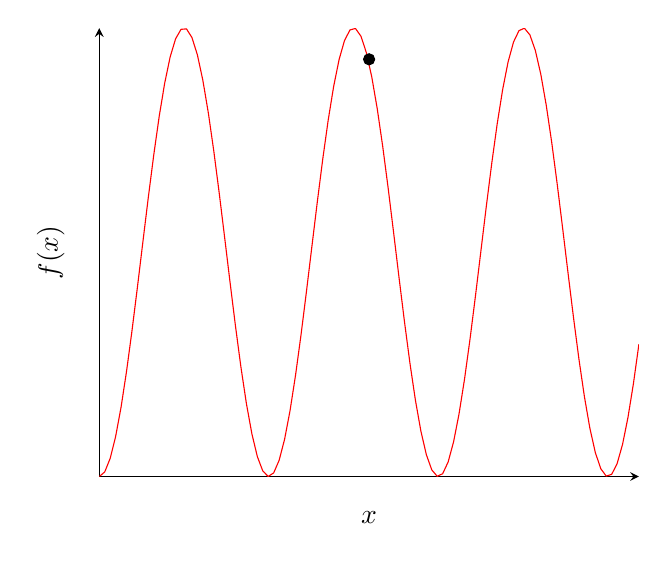
\begin{tikzpicture}
	\begin{axis}[
	    axis lines = left,
	    tick style={draw=none},
	    xticklabels={},
	    yticklabels={},
	    xlabel = $x$,
	    ylabel = {$f(x)$},
	]
	%Below the red parabola is defined
	\addplot [
	    color=red,
	    samples=100,
	]
	{sin(deg(x+5))^2};
    \addplot[mark=*] coordinates {(0,0.93)} node[]{} ;
	\end{axis}
	\end{tikzpicture}  
  \caption{ Non-linear Function\\ with a sample point}
  \label{fig:non_lin_function}
\end{minipage}
\end{figure}

Now, most functions are not constant however it is possible to turn a function into a constant function, and this is exactly what can be done within Monte Carlo integration. To convert a function $f$ to a constant function, a function $f'$ can be introduced which produces the same output as $f$ for every input, but scaled by a constant $c$. The function $f$ is then divided by $f'$ to produce a constant function, as shown in Equation \ref{eq:constant_conversion}.

\begin{equation}
\label{eq:constant_conversion}
\frac{f(x)}{f'(x)} = \frac{1}{c}
\end{equation}

This can be applied to Monte Carlo integration stated in Equation \ref{eq:generalized_mc}, by choosing a probability density function ($pdf$) which produces the same output as $f$ for all inputs, but divided by some normlazing constant factor $c$, keeping $pdf$ as a probability distribution. Therefore, we are able to calculate the true value of the integral thought Monte Carlo integration as shown in Equation \ref{eq:solve_mc_integration}. Where $\frac{1}{c}$ is true value for the integral in Equation \ref{eq:integral}.

\begin{equation}
\label{eq:solve_mc_integration}
\langle F^N \rangle = \frac{1}{N} \sum^{N-1}_{i=0} \frac{f(x)}{pdf(x)} = \frac{1}{N} \sum^{N-1}_{i=0} \frac{f(x)}{cf(x)} =  \frac{1}{N} \sum^{N-1}_{i=0} \frac{1}{c} = \frac{1}{c}
\end{equation}

For most cases it is not possible to know the correct probability distribution function which can convert the Monte Carlo integration problem into integrating a constant function. However, if one has prior knowledge regarding 'important' regions of the functions input space, it is possible to create a probability density function whose shape matches $f$ more closely then a uniform probability distribution. By Important areas of the function input space, I mean areas where when given an input produce a large contribution to the function integral. For example in Figure \ref{fig:improtance_correct}, the most important regions are around the top of the functions peak. 

\begin{figure}[!htb]
\captionsetup{justification=centering}
\minipage{0.32\textwidth}
    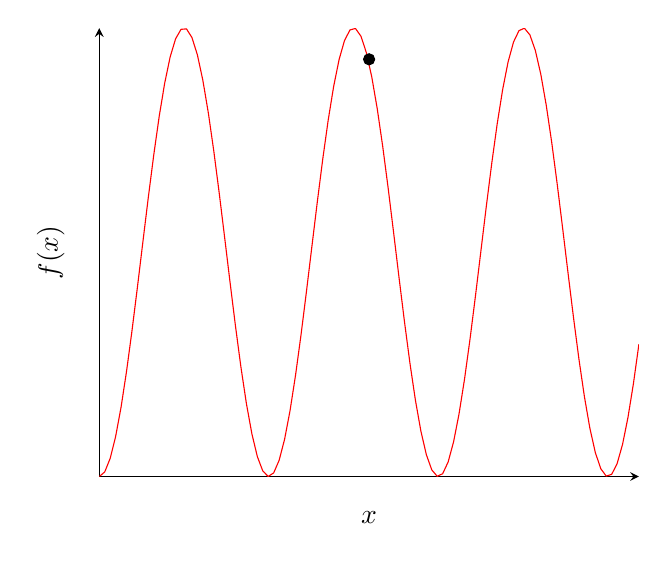
\begin{tikzpicture}
	\begin{axis}[
	    axis lines = left,
	    tick style={draw=none},
	    xticklabels={},
	    yticklabels={},
	    xlabel = $x$,
	    ylabel = {$f(x)$},
	]
	%Below the red parabola is defined
	\addplot [
	    color=red,
	    samples=100,
	]
	{sin(deg(x+5))^2};
    \addplot[mark=*] coordinates {(0,0.93)} node[]{} ;
	\end{axis}
	\end{tikzpicture}  
  \caption{A really Awesome Image}\label{fig:improtance_correct}
\endminipage\hfill
\minipage{0.32\textwidth}
    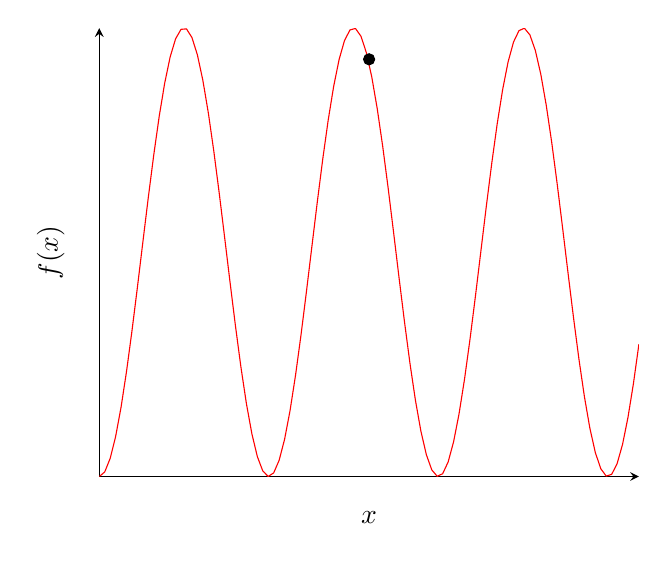
\begin{tikzpicture}
	\begin{axis}[
	    axis lines = left,
	    tick style={draw=none},
	    xticklabels={},
	    yticklabels={},
	    xlabel = $x$,
	    ylabel = {$f(x)$},
	]
	%Below the red parabola is defined
	\addplot [
	    color=red,
	    samples=100,
	]
	{sin(deg(x+5))^2};
    \addplot[mark=*] coordinates {(0,0.93)} node[]{} ;
	\end{axis}
	\end{tikzpicture}  
  \caption{A really Awesome Image}\label{fig:improtance_uniform}
\endminipage\hfill
\minipage{0.32\textwidth}%
    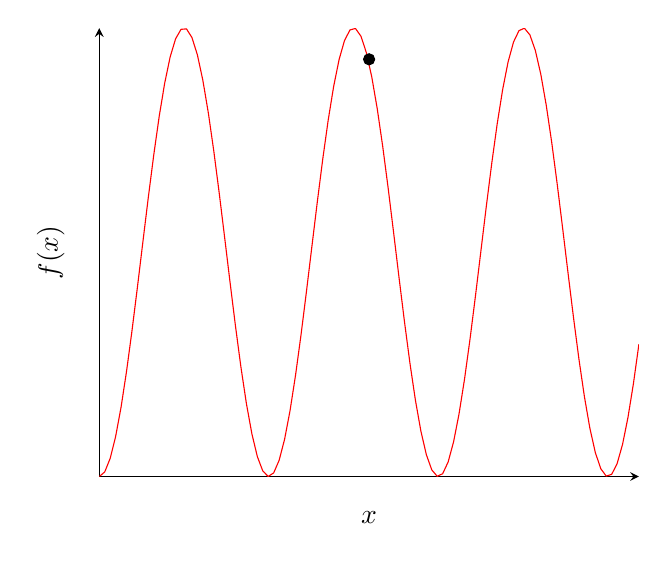
\begin{tikzpicture}
	\begin{axis}[
	    axis lines = left,
	    tick style={draw=none},
	    xticklabels={},
	    yticklabels={},
	    xlabel = $x$,
	    ylabel = {$f(x)$},
	]
	%Below the red parabola is defined
	\addplot [
	    color=red,
	    samples=100,
	]
	{sin(deg(x+5))^2};
    \addplot[mark=*] coordinates {(0,0.93)} node[]{} ;
	\end{axis}
	\end{tikzpicture}  
  \caption{A really Awesome Image}\label{fig:improtance_incorrect}
\endminipage
\end{figure}

As previously explained, Figure\ref{fig:improtance_correct} represents a probability density function which has a similar shape to the function which is being integrated. Therefore the variance in the Monte Carlo integration approximation will be lower then that of the uniform distribution shown in Figure \ref{fig:improtance_uniform}. Figure \ref{fig:improtance_incorrect} presents an example where the created probability density function does not resemble the shape of the function which is being integrated. Using this $pdf$ in Monte Carlo integration in this case will actually increase the variance in the output compared to that from a uniform $pdf$ shown in Figure \ref{fig:improtance_uniform}.  This is due to regions which have high importance according to the $pdf$ are actually less important regions for the function $f$, meaning areas of the input space receive incorrect contribution weighting, causing the variance in the Monte Carlo integration approximation to rise.


\section{Markov Decision Processes and TD-Learning}

\section{Linking TD-Learning and Light Transport Simulation}

\section{The expected SARSA Path tracer}

\begin{comment}
{\bf A compulsory chapter,     of roughly $10$ pages} 
\vspace{1cm} 

\noindent
This chapter is intended to describe the technical basis on which execution
of the project depends.  The goal is to provide a detailed explanation of
the specific problem at hand, and existing work that is relevant (e.g., an
existing algorithm that you use, alternative solutions proposed, supporting
technologies).  

Per the same advice in the handbook, note there is a subtly difference from
this and a full-blown literature review (or survey).  The latter might try
to capture and organise (e.g., categorise somehow) {\em all} related work,
potentially offering meta-analysis, whereas here the goal is simple to
ensure the dissertation is self-contained.  Put another way, after reading 
this chapter a non-expert reader should have obtained enough background to 
understand what {\em you} have done (by reading subsequent sections), then 
accurately assess your work.  You might view an additional goal as giving 
the reader confidence that you are able to absorb, understand and clearly 
communicate highly technical material.
\end{comment}

\subsection{Plan}
\textbf{Breakdown}

\begin{itemize}
\item The rendering equation and what each component is, how this relates to global illumination

\item Path tracings use of the rendering equation. How monte carlo comes into play. The iterative version of the path tracing algorithm. Concept of a light path.

\item Importance sampling in terms of BRDF and relating this to reducing variance in pixel colours leading to less noise via a reduction in variance, but incorrect importance sampling can do the opposite. Give examples of classical importance sampling techniques and their performance. Critic them and clearly present where their shortcomings are and how they are unavoidable.

\item Introduce reinforcement learning: Markov Decision Process, Bellman 
Equation, Temporal Difference Learning and its strong points and weaknesses,
 how does it differ to traditional monte-carlo (might not be relevant). Proved 
 to converge on the true valuation function for a given state-action pair when 
 run infinitely
 
 \item Give Nvidia's derivation of their learning rule. How does the Markov Decision Process relate to a rendered scene, i.e. what is the AI doing for us here. Provide a justification of parameter matching. Essentially cover all reinforcement learning theory of the paper here, with a justification (mathematical) and visual examples of why it works. 
 
 \item Discretizing the state space is required for Q-learning to be applied, shortcoming is that it may not work very well with infinite state spaces. Introduce the Irradiance volume and how it can be used to rather store actual irradiance values to instead store Q-values. The irradiance distribution for a given point in the scene. Sampling the irradiance volumes around the scene onto geometry. 
 
 \item Present the full algorithm proposed by Nvidia, displaying irradiance volumes learned Q-values (as an image of hemispheres) throughout the process and stating how these update a cumulative distribution to sample from.
 
 \item Introduce concept of Deep Q-learning and how it no longer needs a discretized state space. However it still requires action space to be discretized (unlike an actor-critic setup). What is the role of the network and what other function approximators can be trialled. Explain in quite some detail the DeepMind Atari paper which introduced Deep Reinforcement learning.
 
\end{itemize}

\textbf{Preliminary}
\begin{enumerate}
\item Define what a ray-tracing rendering algorithm consists of and the difference 
between global and direct illumination. Acknowledge other ray-tracing algorithm l
ike bi-directional path-tracers, Rendermans algorithm, photon mapping. 

\item Define terms like BRDF, radiance, irradiance and the rendering equation

\item Explain the details of the path-tracing algorithm in depth. It should be 
completely clear the relation between path-tracing and the rendering equation. 
It should be clear where the Monte Carlo approach comes in and why 
importance sampling within path-tracing can yield less noisy and more accurate
 results, potentially in the same fixed time-budget

\item Introduce the concept of importance sampling in computing global 
illumination with some early examples of its success, use in industry and recent 
papers on efficient light transport simulation. State the reasoning behind why
it still continues to accurately simulate global illumination, in other words, why
zero-contribution light paths do not contribute to the image.

\item Introduce reinforcement learning: Markov Decision Process, Bellman 
Equation, Temporal Difference Learning and its strong points and weaknesses,
 how does it differ to traditional monte-carlo (might not be relevant). Proved 
 to converge on the true valuation function for a given state-action pair when 
 run infinitely

\item State the derived learning rule supplied by Ken Dahm and visualize the 
matching terms as well as a justification why each parameter matches. What 
is the value and the incentive, diminishing return for rewards far in the future etc

\item State new on-line algorithm proposed by Ken Dahm and details for 
discretizing the state and action space into the Irradiance Volume data-structure
 which was previously introduced 

\item Introduce the concept of deep reinforcement learning, describing how
 DeepMind used the technique for playing Atari games. Given a state give me 
 the state-action values for all actions possible in that state.  Then how we 
 can apply this to our scene to model the state space and continuous.
 
 

\end{enumerate}

% -----------------------------------------------------------------------------

\chapter{Deep Q-Learning Path tracer}
\label{chap:deep-q}

\begin{comment}
{\bf A topic-specific chapter, of roughly $15$ pages} 
\vspace{1cm} 

\noindent
This chapter is intended to describe what you did: the goal is to explain
the main activity or activities, of any type, which constituted your work 
during the project.  The content is highly topic-specific, but for many 
projects it will make sense to split the chapter into two sections: one 
will discuss the design of something (e.g., some hardware or software, or 
an algorithm, or experiment), including any rationale or decisions made, 
and the other will discuss how this design was realised via some form of 
implementation.  

This is, of course, far from ideal for {\em many} project topics.  Some
situations which clearly require a different approach include:

\begin{itemize}
\item In a project where asymptotic analysis of some algorithm is the goal,
      there is no real ``design and implementation'' in a traditional sense
      even though the activity of analysis is clearly within the remit of
      this chapter.
\item In a project where analysis of some results is as major, or a more
      major goal than the implementation that produced them, it might be
      sensible to merge this chapter with the next one: the main activity 
      is such that discussion of the results cannot be viewed separately.
\end{itemize}

\noindent
Note that it is common to include evidence of ``best practice'' project 
management (e.g., use of version control, choice of programming language 
and so on).  Rather than simply a rote list, make sure any such content 
is useful and/or informative in some way: for example, if there was a 
decision to be made then explain the trade-offs and implications 
involved.

\section{Example Section}

This is an example section; 
the following content is auto-generated dummy text.
\lipsum

\subsection{Example Sub-section}

\begin{figure}[t]
\centering
foo
\caption{This is an example figure.}
\label{fig}
\end{figure}

\begin{table}[t]
\centering
\begin{tabular}{|cc|c|}
\hline
foo      & bar      & baz      \\
\hline
$0     $ & $0     $ & $0     $ \\
$1     $ & $1     $ & $1     $ \\
$\vdots$ & $\vdots$ & $\vdots$ \\
$9     $ & $9     $ & $9     $ \\
\hline
\end{tabular}
\caption{This is an example table.}
\label{tab}
\end{table}

\begin{algorithm}[t]
\For{$i=0$ {\bf upto} $n$}{
  $t_i \leftarrow 0$\;
}
\caption{This is an example algorithm.}
\label{alg}
\end{algorithm}

\begin{lstlisting}[float={t},caption={This is an example listing.},label={lst},language=C]
for( i = 0; i < n; i++ ) {
  t[ i ] = 0;
}
\end{lstlisting}

This is an example sub-section;
the following content is auto-generated dummy text.
Notice the examples in Figure~\ref{fig}, Table~\ref{tab}, Algorithm~\ref{alg}
and Listing~\ref{lst}.
\lipsum

\subsubsection{Example Sub-sub-section}

This is an example sub-sub-section;
the following content is auto-generated dummy text.
\lipsum

\paragraph{Example paragraph.}

This is an example paragraph; note the trailing full-stop in the title,
which is intended to ensure it does not run into the text.

\end{comment}

\subsection{Plan}

% I imagine this section to be like a mini paper starting at new method

\textbf{Breakdown}
\begin{enumerate}

\item State learning rule for deep Q-learning and the difference from deep Q-learning to q-learning. Maybe some of the difficulties associated with deep q-learning versus q-learning, and some of the general advantages. 

\item Derive the learning rule for deep q-learning network which I used, once again justifying terms throughout the derivation.

\item Explain concept of eta-greedy policy used. Explain exploration vs exploitation but we will talk about this more later

\item Describe how the current method is used for diffuse surfaces. Introduce the pseudo code for the new algorithm. Give a description of each stage and what it does. Relating back to properties such as bias rendering and pointing out assumption made by the path tracer.

\item Present and explain the network architecture. Explain in depth about how the state was modelled as a point relative to all vertices to give the network information about the position of the vertex relative to the rest of the world compared to passing in a single position. Relate this to Atari games, we get an image showing where we are relative to the world rather than just a single position in the world.

\item Present some results side by side against a default path tracer and Nvidia's reinforcement learning approach. Pointing out aspects of the image and reasoning for certain parts.

\end{enumerate}

% -----------------------------------------------------------------------------

\chapter{Critical Evaluation}
\label{chap:evaluation}

{\bf A topic-specific chapter, of roughly $15$ pages} 
\vspace{1cm} 

\noindent
This chapter is intended to evaluate what you did.  The content is highly 
topic-specific, but for many projects will have flavours of the following:

\begin{enumerate}
\item functional  testing, including analysis and explanation of failure 
      cases,
\item behavioural testing, often including analysis of any results that 
      draw some form of conclusion wrt. the aims and objectives,
      and
\item evaluation of options and decisions within the project, and/or a
      comparison with alternatives.
\end{enumerate}

\noindent
This chapter often acts to differentiate project quality: even if the work
completed is of a high technical quality, critical yet objective evaluation 
and comparison of the outcomes is crucial.  In essence, the reader wants to
learn something, so the worst examples amount to simple statements of fact 
(e.g., ``graph X shows the result is Y''); the best examples are analytical 
and exploratory (e.g., ``graph X shows the result is Y, which means Z; this 
contradicts [1], which may be because I use a different assumption'').  As 
such, both positive {\em and} negative outcomes are valid {\em if} presented 
in a suitable manner.

\subsection{Plan}

\textbf{Data to collect}
\begin{itemize}

\item Build 4 different scenes:

\begin{itemize}
\item Simple geometry, Indirectly illuminated scene: Here both reinforcement learning methods should perform excellently

\item Simple geometry, Directly illuminated scene: Here all methods should perform well

\item Complex geometry, Indirectly illuminated scene: Can both methods do this - will take a lot of training, deeper NN potentially

\item Complex geometry, Directly illuminated scene: Can both methods do this - will take a lot of training, deeper NN potentially
\end{itemize}

\item Number zero-contribution light paths/ light paths that do not intersect with a with a light after $n$ bounces therefore they become irrelevant for all methods with accumulated frames on the x-axis

\item Variance in points around the room to train network in order to make training batches as varied as possible (this is a weird one, essentially assessing the fact that we do not need a replay buffer).

\item eta-greedy constant for loss curve for training the network \& decaying eta-greedy policy graph for the loss as well

\item Visual representation of Q-values being higher in directions near light source: Map q-values to hemispheres in the scene and get a close up, clearly indicating its ability to sample in the correct direction

\item 1 SPP, 16 SPP, 32 SPP, 64 SPP, 128 SPP, 256 SPP for all three methods on 4 different scenes to evaluate their effectiveness: Assessing accuracy of global illumination approximation

\item Limitations: Number of angles which can accurately be learned by the network, accuracy  needs to be compared with expected SARSA approach for a single radiance volume at a given point in the scene. Size of the scene which can be learnt accurately.

\end{itemize}

\textbf{Preliminary}
\begin{enumerate}
\item Exploration vs Exploitation for both techniques, exploration can yield to better results plus exploitation does not accurately simulate light, relate to the rendering equation and how light works in the physical world.

\item Show for about 4 different scenes the results for a $n$ different numbers of samples; the images, average path length, number of light paths which actually contribute to the image which are sampled between all techniques. I will have to analyse which reduces the number of zero contribution paths the most, but also still assess if the image is photo-realistic.

\item Also analyse default Q-learnings ability on top of expected SARSA

\item Justify reasoning for choosing to analyse Q-Learning, Expected SARSA and DQN (because they have good results for other cases and TD learning fits the online learning procedure)

\item Assess the number of parameters required, configuration is important for these algorithms, if it is very difficult to get right, then the time spent configuring may not be worth it compared to actually rendering the image. E.g. default path-tracing there are not other parameters apart from the number of samples per pixel, expected SARSA requires the user to specify the memory which is allowed to be used by the program, this requires careful consideration, as well as the threshold the distribution cannot fall below, the deep Q-learning algorithm requires less config but potentially different neural network architectures should be investigated to further reduce the number of zero-contribution light paths. 

\item Ease of implementation 

\item Parallelisability of each algorithm, path-tracing is far easier to parallelise as it requires minimal memory accesses by the program to infer pixel values, as opposed to expected SARSA which requires many. Deep-q learning has more customizability in terms of parallelizing (needs more research)

\item Memory usage: Path-tracing is minimal, Expected SARSA is unbounded, Deep Q-Learning is bounded by the size of the neural network, but the memory it requires is still significant (needs more research)

\item DQN vs Expected Sarsa: Do not have to wait for an iteration to begin
 importance sampling on the newly learned Q values for a given point, 
 neural network is continually trained and inferred from. Continuous state 
 space vs discretized required for storage in expected SARSA.
\end{enumerate}

% -----------------------------------------------------------------------------

\chapter{Conclusion}
\label{chap:conclusion}

{\bf A compulsory chapter,     of roughly $5$ pages} 
\vspace{1cm} 

\noindent
The concluding chapter of a dissertation is often underutilised because it 
is too often left too close to the deadline: it is important to allocation
enough attention.  Ideally, the chapter will consist of three parts:

\begin{enumerate}
\item (Re)summarise the main contributions and achievements, in essence
      summing up the content.
\item Clearly state the current project status (e.g., ``X is working, Y 
      is not'') and evaluate what has been achieved with respect to the 
      initial aims and objectives (e.g., ``I completed aim X outlined 
      previously, the evidence for this is within Chapter Y'').  There 
      is no problem including aims which were not completed, but it is 
      important to evaluate and/or justify why this is the case.
\item Outline any open problems or future plans.  Rather than treat this
      only as an exercise in what you {\em could} have done given more 
      time, try to focus on any unexplored options or interesting outcomes
      (e.g., ``my experiment for X gave counter-intuitive results, this 
      could be because Y and would form an interesting area for further 
      study'' or ``users found feature Z of my software difficult to use,
      which is obvious in hindsight but not during at design stage; to 
      resolve this, I could clearly apply the technique of Smith [7]'').
\end{enumerate}

\subsection{Plan}
\begin{enumerate}
\item Summarise contributions:

\begin{enumerate}
\item Implementing a path tracer from scratch to analyse in depth the difficulties and issues that come with Ken Dahm's algorithm. Including memory usage, parallelisation and parameter usage.

\item Analysis of different reinforcement learning approaches pitched together clearly on a variety of scenes

\item Analysis of neural networks ability to learn the irradiance distribution function

\item Online deep-reinforcement learning algorithms effectiveness of learning irradiance distribution function
\end{enumerate}

\item If DQN does not work well provide some further analysis on potential other alternatives which could be used.

\item Future Work: Policy learning to model continuous action \& state space

\item DDQN and other deep reinforcement learning strategies
\end{enumerate}

% =============================================================================

% Finally, after the main matter, the back matter is specified.  This is
% typically populated with just the bibliography.  LaTeX deals with these
% in one of two ways, namely
%
% - inline, which roughly means the author specifies entries using the 
%   \bibitem macro and typesets them manually, or
% - using BiBTeX, which means entries are contained in a separate file
%   (which is essentially a databased) then inported; this is the 
%   approach used below, with the databased being dissertation.bib.
%
% Either way, the each entry has a key (or identifier) which can be used
% in the main matter to cite it, e.g., \cite{X}, \cite[Chapter 2}{Y}.

\backmatter

\bibliography{dissertation}

% -----------------------------------------------------------------------------

% The dissertation concludes with a set of (optional) appendicies; these are 
% the same as chapters in a sense, but once signaled as being appendicies via
% the associated macro, LaTeX manages them appropriatly.

\appendix

\chapter{An Example Appendix}
\label{appx:example}

Content which is not central to, but may enhance the dissertation can be 
included in one or more appendices; examples include, but are not limited
to

\begin{itemize}
\item lengthy mathematical proofs, numerical or graphical results which 
      are summarised in the main body,
\item sample or example calculations, 
      and
\item results of user studies or questionnaires.
\end{itemize}

\noindent
Note that in line with most research conferences, the marking panel is not
obliged to read such appendices.

% =============================================================================

\end{document}
